% !TeX spellcheck = zh_CN
\documentclass[aps,pre,12pt,preprint,%
	onecolumn,showpacs,showkeys,nofootinbib]{revtex4-1}
%UnlimitedFonts
	\def\hmmax{0}
	\def\bmmax{0}
%SVG
	\usepackage{svg}
%Tables
	\usepackage{array,booktabs,tabularx,multirow}
	\newcolumntype{C}[1]{>{\hsize=#1\hsize%
		\centering\arraybackslash}X}
%Math&Fonts
	\let\latexointop\ointop
	\usepackage{mathtools,amssymb,bm % basics
		,physics,siunitx,slashed % physics
		,esint,nicefrac,extarrows,mathrsfs % more symbols
		,calligra,romannum,dsfont,fourier-orns % nice fonts
		,eqnarray,resizegather,empheq % more envs
		,relsize,stackengine % utils
	}
%	\usepackage{amsthm}
	\usepackage[scr=esstix]{mathalfa}
	\usepackage[only,sslash]{stmaryrd}
	%DisplaySetup
	\newcommand*\bbox[1]{\fbox{\hspace{1em}\addstackgap[5pt]{#1}\hspace{1em}}}
	\empheqset{box=\bbox}
	\mathtoolsset{showonlyrefs}
%Utils
	%Legacy \oint
	\let\ointop\undefined
	\let\ointop\latexointop
	%Calligra
	\DeclareMathAlphabet{\mathcalligra}{T1}{calligra}{m}{n}
	\DeclareFontShape{T1}{calligra}{m}{n}{<->s*[2.2]callig15}{}
	%CosmeticTweaks
	\newcommand\inlineeqno{\stepcounter{equation}\ (\theequation)}
	\newcommand\scalemath[2]{\scalebox{#1}{\mbox{\ensuremath{\displaystyle #2}}}}
	\newcommand\raisemath[2]{\raisebox{#1\depth}{${#2}$}}
	\newfontfamily\signature{Vladimir Script}
	\newcommand{\newparagraph}{\pagebreak[3]
		\noindent\hfil%
		\raisebox{-4pt}[10pt][10pt]{\leafright~\qquad~\leafleft}%
		\par\nopagebreak%
	}
%CustomCmds
	%Brackets
	\DeclarePairedDelimiter\ave{\langle}{\rangle}
	\DeclarePairedDelimiterX\inprod[2]{\langle}{\rangle}{#1,#2}
	%Basics
	\newcommand{\mbb}[1]{\mathbb{#1}}
	\newcommand{\mrm}[1]{\mathrm{#1}}
	\newcommand{\mcal}[1]{\mathcal{#1}}
	\newcommand{\mscr}[1]{\mathscr{#1}}
	\newcommand{\tup}[1]{\textup{#1}}
	\newcommand{\mop}[1]{\operatorname{#1}}
	%Extras
	\newcommand{\scriptr}{\mathcalligra{r}\,}
	\newcommand{\rvector}{\pmb{\mathcalligra{r}}\,}
	\newcommand{\hodgedual}{\operatorname{\star}}
	\newcommand{\dual}{\ \xlongleftrightarrow{\ \textrm{dual}\ }\ }
	\newcommand{\idty}{\mathds{1}}
	\newcommand{\proj}[1]{\operatorname{%
		proj_{\mathit{#1}}}}
	\newcommand{\propsim}{\mathbin{\ensurestackMath{
		\stackunder[2pt]{\propto}{\sim}
	}}}
	\newcommand{\textbox}[1]{\fbox{#1}}
	\newcommand{\pdd}[1]{\operatorname{\partial_{\mathnormal{#1}}}}
	\newcommand{\cdd}{\operatorname{D}\!}
	\newcommand{\cdv}[1]{\operatorname{%
		\nabla_{\!\mathit{#1}\!}}}
	\newcommand{\ldv}[1]{\operatorname{%
		\mcal{L}_{\!\mathit{#1}\!}}}
	\newcommand{\ric}[1]{\operatorname{%
		Ric}\!\pqty{#1}}
%Hacks
	% physics.sty <texmf-dist/tex/latex/physics/>
	% USER: more spacing around Dirac's middle vert
	\newcommand{\xmiddle}[1]{\mspace{1mu}\middle#1\mspace{1mu}}
	\DeclareDocumentCommand\innerproduct{ s m g }
	{ % Inner product
		\IfBooleanTF{#1}
		{ % No resize
			\IfNoValueTF{#3}
			{\vphantom{#2}\left\langle\smash{#2}\xmiddle\vert\smash{#2}\right\rangle}
			{\vphantom{#2#3}\left\langle\smash{#2}\xmiddle\vert\smash{#3}\right\rangle}
		}
		{ % Auto resize
			\IfNoValueTF{#3}
			{\left\langle{#2}\xmiddle\vert{#2}\right\rangle}
			{\left\langle{#2}\xmiddle\vert{#3}\right\rangle}
		}
	}

%Miscellaneous
%	\newcommand{\tabindent}{\hspace{2em}}
	\newcommand{\cuSample}{$\mrm{CuSO_4}$溶液}
	\newcommand{\perc}[1]{\SI{#1}{\percent}}
\begin{document}
%Basic Data
	\title{%
	\texstringonly{\hfil\\[2\baselineskip]}
	\sf\LARGE%
		脉冲磁共振及核磁共振成像%
	\texstringonly{\vspace{3ex}}}
	\author{\fangsong\large%
		Bryan%
	\vspace{2mm}}
	\affiliation{\it%
		北京大学物理学院~~学号:\normalfont 1500066666\,}
	\date{\today}
	\keywords{核磁共振\ 脉冲磁共振\ 自由感应衰减\ 自旋回波\ 核磁共振成像编码}
	\email{masked_email_please_contact@github.com}

\begin{abstract}
\vspace{10mm}
\begin{spacing}{1.5}\normalsize
\setlength{\parskip}{.3\baselineskip}
%	200—300字,
%	说明用什么方法做了什么事,
%	由此得到什么结果和结论,
%	有何意义.
%	不用缩略词,不用第一人称.
%%%%%%%%%%%%%%%%%%%%%%%%%%%%%%%%
	本实验检验了脉冲磁共振的基本原理,探索了其在核磁共振成像方面的基础应用,利用JXMRI-S2.1型磁共振成像仪以自旋回波成像法获取了 \cuSample 的核磁共振图像。
	
	在此基础上,通过在 \cuSample 中加入正三角形、正六边形样品后成像,检验了该成像方案的分辨能力;并通过对比不同浓度的 \cuSample 像,初步验证了$T_2$加权成像原理。
\end{spacing}
\end{abstract}

\maketitle
\thispagestyle{titlepagestyle}

%%  课程实验报告应假定读者既不是已知全部实验细节的指导教师,也不是缺少专业知识的公众,而是同领域的实验研究者,或审稿人. 不能要求读者要在读过课程讲义后才能读懂课程实验报告.
%%  凡不是自己独立思考得到的内容都应该引参考文献. 不能大段引用同一参考文献. 对复杂问题,应该优先考虑引用参考文献得到结果. 对简单一些的问题才鼓励独立思考.
\section{引言}
%%	研究论文引言一般包含以下内容:
%%	(1)所研究领域背景和现状;
%%	(2)有待研究的问题;
%%	(3)本研究的目的、主要内容和结果;
%%	(4)结果的意义.\par
%%	在写实验报告的引言时,同学可以假想自己是第一个做类似研究的人.\par
%%	引言一定要切合报告正文,不能漫无目的地介绍背景. 要快速地将读者引导到报告主题上,并作较深入的讨论.\par
%%	引言篇幅可以在较大范围内变化,但最长不应超过报告文字篇幅的1/3.\par
%%	引言撰写可以参考实验讲义,可以复述,但不能复制讲义上的任何一句话.\par
%%%%%%%%%%%%%%%%%%%%%%%%%%%%%%%
\vspace{-1ex}
	核磁共振(nuclear magnetic resonance, NMR)是核磁矩与特定频率的射频场发生共振吸收的现象;激发核与通过相互作用辐射退激,共振频率和退激的时间尺度与物质种类、结构和环境有关,故可利用核磁共振探测物质的结构;通过额外的空间编码,则可用于物质成像,此即核磁共振成像(NMR imaging, NMRI)的基本原理。
	
	1971年美国化学家P. C. Lauterbur提出了核磁共振成像的可行思路和方法,其工作 \cite{lauterbur1973image} 于1973年发表于《自然》杂志,奠定了现代核磁成像基础的基础。在P. Mansfield等人的改进下,NMRI技术不断得到优化,并被广泛应用于医学成像中;NMRI对人体没有电离辐射损伤,且分辨率高、对比度大。Lauterbur与Mansfield因其在核磁共振成像方面的贡献被授予2003年诺贝尔医学奖。
	
	NMRI的关键是需要对核磁共振信号进行空间编码,解译经过编码的NMR信号以得实空间的NMR图像,可见编码方式是NMRI技术的核心。本实验即在了解脉冲磁共振原理的基础上,探索了基本的空间编码方式。
\vspace{-2ex}
\section{理论}
\vspace{-1ex}
%\setlength{\jot}{0pt}
	核磁共振方法有稳态核磁共振和脉冲核磁共振两种,应用于成像时则基本采用脉冲磁共振的方法。具体而言,脉冲核磁共振通过探测核磁系统对短时射频脉冲的响应确定系统的共振特性;设脉冲强度$B'$, 作用时间为$\tau$, 则核磁矩偏离平衡位置:
	\begin{equation}
		\theta = \gamma B'\tau
	\end{equation}
	其中$\frac{\gamma}{2\pi} = \frac{g\mu_N}{2\pi\hbar}$为回旋频率。
	
	此后,经过一段时间的驰豫,磁化强度指数衰减$M_{xy}\to 0,\,M_z\to M_0$, 纵向($z$)、横向($xy$)驰豫时间分别记为$T_1,\,T_2$, 由于$M_z = M_0$时必有$M_{xy} = 0$, 而反之不然,故有$T_2 < T_1$. 
\clearpage
	
	利用感应线圈,可检测、分析驰豫过程的自由感应衰减信号(free inductive decay, FID),傅立叶分析以得到共振信息。
	
	特别地,若加$\theta = \frac{\pi}{2}$射频脉冲,使$\vb{M} = M_0\,\hat{\vb{z}}$倒向$xy$平面,经历一段时间$\tau$后核磁矩相位离散使得$M_{xy} \simeq 0$, 此时再加$\pi$脉冲可实现重新聚相,得到自旋回波信号(spin echo, SE)。本实验中成像时探测的信号即为自旋回波信号。
	
	为实现成像目的,须对核磁共振信号进行空间编码;这通过附加线性梯度场$\vb{B}(x,y,z) \sslash \hat{\vb{z}}$实现。具体而言,
	\begin{enumerate}[label=\arabic*.]
	\item \textbf{$z$选层:}加$B_z = zG_z$, 此时有共振条件:
	\begin{equation}
		\omega = \omega(z) = \gamma\,(B_0 + G_z z)
	\end{equation}
	脉冲带宽$\Delta\omega$限定了$\omega$的取值范围,此时只有特定$z = z_0$横断面附近的核将产生共振,其他各层的核均处于非共振状态,对NMR信号无贡献。
	\item \textbf{$y$相位编码:}撤去脉冲、$G_z$后,加$B_z = yG_y$使不同$y$处的核磁矩以不同角频率进动,持续$t_y$, 可使不同$y$处附加不同的相位:
	\begin{equation}
		\omega_y t_y = \gamma\,G_y\,y\,t_y
	\end{equation}
	即实现了$y$方向的编码。
	\item \textbf{$x$频率编码:}加$B_z = xG_x$, 类似相位编码,有:
	\begin{equation}
		\omega_x t_x = \gamma\,G_x\,x\,t_x
	\end{equation}
	即实现了$x$方向的编码。
	\end{enumerate}
	
	至此,便完整地实现了空间编码;注意$x,y$方向的编码原理稍有差异,具体而言,$\omega_x(x)$可直接由感应信号$S(t) = S(t_x - t_0)$傅立叶变换得到,故称为频率编码;相反,$y$方向的信息须通过改变$G_y t_y$多次脉冲得到,故为相位编码。
\clearpage
	
	考虑改变$t_y$多次脉冲得到的序列$S(t_x,t_y) = S(t)|_{t_y}$, 有:
	\begin{equation}
		S(t_x, t_y) \propto \iint\dd{x}\dd{y}
			e^{i\omega_x t_x} e^{i\omega_y t_y}
			\rho(x,y)\,
			\exp(-\frac{t}{T_2})
	\end{equation}
	这里$\omega_x t_x,\,\omega_y t_y$正是编码时附加的相位,注意$t, t_x$线性相关;对$S(t_x, t_y)$进行二维傅立叶变换,即得$T_2$加权的核密度$\tilde{\rho}(x,y)$. 此即成像的基本原理。
%\restorejot
%%%%%%%%%%%%%%%%%%%%%
\section{实验装置}
\vspace{0\baselineskip}
%%	在此部分需要将实验条件交待清楚到别人能重复你的实验结果的程度. 此外,还需表明你已尽了最大努力来提高实验精度和结果的可靠性. 简单的不确定度估计可以在此节给出,复杂一些的可以放到分析讨论部分.\par
%%	实验条件不仅是指直接影响实验结果的实验参量,而且还包括影响实验质量和可靠性的因素,如室温、空气湿度、基真空、原材料纯度等.\par
%%	作为教学实验报告,此节写详细一点没有坏处.\par
%%	成段有叙述,必要才分节。
%%%%%%%%%%%%%%%%%%%%%%%%%%%%%%%
	实验采用JXMRI-S2.1型磁共振成像仪及相应的自动化控制软件,由三组梯度线圈实现信号的空间编码;使用前仪器须开机预热$\sim\SI{1}{\hour}$. 样品与磁场的相对位置如图所示;约定恒磁场沿$z$方向,则选层梯度沿$x$方向,即附加$\vb{B}(x,y,z) = xG_x\,\hat{\vb{z}}$, 相应地相位、频率梯度分别沿$y,z$方向。
	\begin{figure}[!ht]
	\centering
	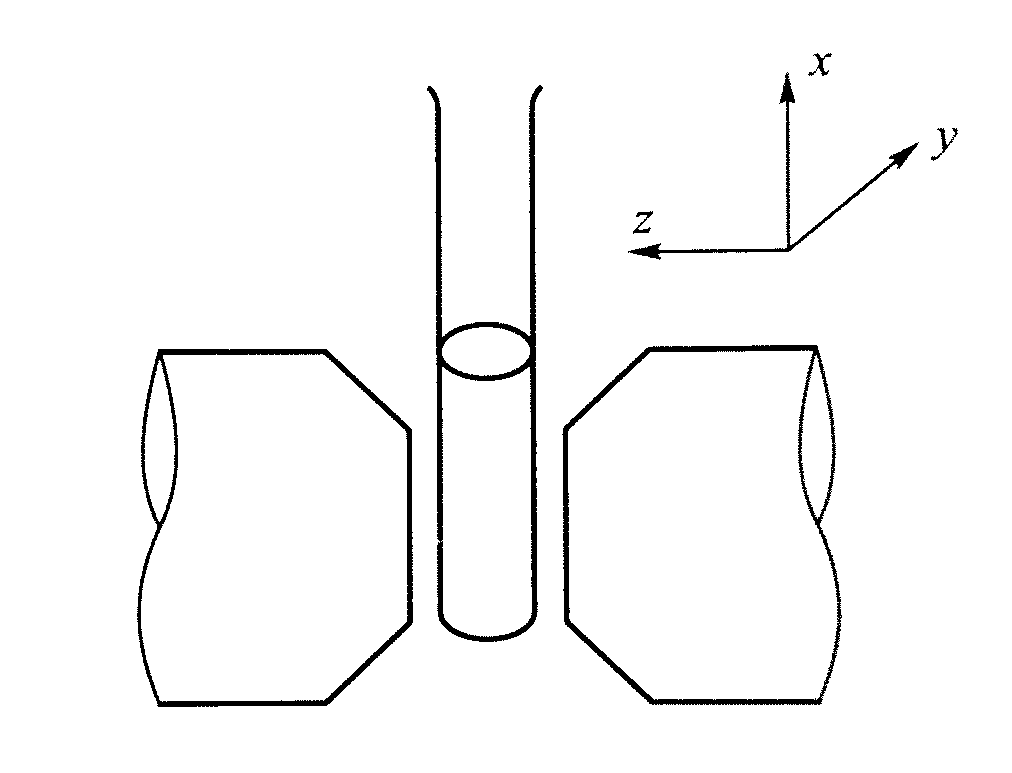
\includegraphics[width=.5\linewidth]{img/scheme.png}
	\caption{磁场与样品的空间坐标约定示意图,选自 \cite{textbook}. }
%	\begin{explain}
%		NULL
%	\end{explain}
	\end{figure}
	
	实验中采用(\textit{截断的})时域包络$\sim \sinc\alpha = \frac{\sin\alpha}{\alpha}$的软脉冲激发原子核并获取自旋回波信号。软脉冲在频域为矩形脉冲,即带宽$\Delta\omega$内各频率强度相同,由于空间编码后共振频$\omega$带有空间信息,采用软脉冲可减少成像时的密度偏差。
\clearpage
\section{结果与分析}
%	实验结果应尽量以图表的形式给出. 每一个图表都应该是完整的,即阅读图表时可以不必依赖正文.\par
%	依自己意愿,实验结果和对结果的分析讨论既可分为两节也可合在一节.\par
%
%	每个图一般包含:图名、轴名、轴、刻度、标尺、数据点、曲线、图例、标注和图注等部分. 应尽量让读者不看正文就能基本理解图的含意.\par
%	逐点测量得到的函数关系要同时用表格和图给出. 需要作比较的多条曲线要画在同一图上.\par
%	为避免读者在图表和正文间反复跳跃阅读,在正文中也要对图表作必要的说明.\par
%
%	对于预料之外的实验结果,必须首先小心证明其可靠性.读者只有在相信你的实验结果时才愿意花时间看你的分析.\par
%	必须用文字归纳整理出正式的实验结果或结论.可信的实验结果是课程报告最重要的内容.作为一个实验物理工作者,分析解释出错并不丢脸,实验结果不被采信则是致命的.\par
%	教学实验的结论往往是预先知道的. 所以,教师更关心的是你的说理过程. 一般说来,单由课内实验的结果不足以能得到明确的结论. 此时,你可以引用他人的研究结果来帮助帮助自己的论证,但必须注明出处. \par
%	确实不能得到明确结论时,可以给出几种可能结论并指出可以再做哪些实验来帮助作进一步的判断.\par
%	总之,分析讨论部分要做到: 论据要valid,论证要reasonable,结论要convincing.\par
%%%%%%%%%%%%%%%%%%%%%%%%%%%%%%
\vspace{-1ex}
	实验前首先选用硬脉冲校准质子共振激发频率,作为后续脉冲的中心频率。实验过程中由于永磁体的磁场强度随温度波动,在每次成像前均应重校激发频率。装入样品 \perc{.5} \cuSample, 初次校准得到的修正激发频率为:
	\begin{equation}
		f = \SI{12.705383}{\MHz}
	\end{equation}
	随后切换为软脉冲,观察自由感应衰减信号,通过比较不同参数时的信号强度以确定$\frac{\pi}{2},\pi$脉冲对应的最佳参数。
	
	本实验中固定脉冲宽度$\tau = \tup{D1} = \SI{1000}{\us}$, 通过调整幅度$B' \propto \tup{D1P}$以获取$\frac{\pi}{2},\pi$脉冲。实测FID信号的首个极大、极小分别对应$\tup{D1P} \sim 22, 41$, 分别对应$\frac{\pi}{2},\pi$脉冲。以此为参考值设定成像部分$\tup{D1P}, \tup{D2P}$参数。
	
	在此基础上,设置采样率$\tup{NS} = 16$, 重校频率后以自旋回波法成像,得:
	\begin{figure}[!ht]
	\centering
	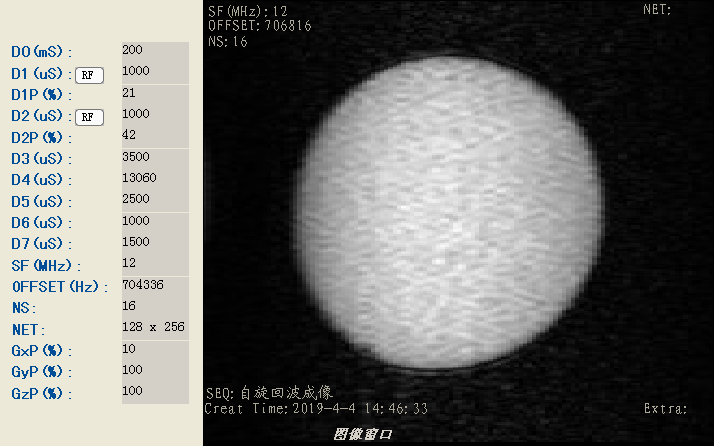
\includegraphics[width=.8\linewidth]{img/plots/sample0.png}
	\caption{\perc{.5} \cuSample $x = 0$截面核磁共振图像及相应参数}
	\vspace{-1ex}
	\end{figure}
\FloatBarrier\noindent%
	随后在试管中加入正三角形、正六边形样品,重校频率、再次成像,结果如下。
\clearpage
	
	\begin{figure}[!ht]
	\vspace{-2ex}
	\centering
	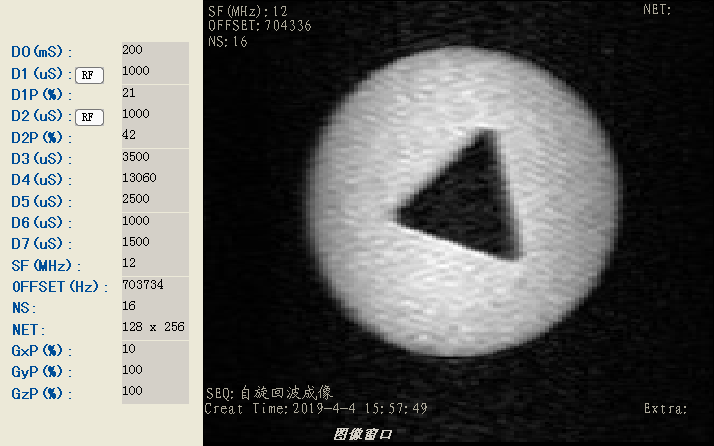
\includegraphics[width=.78\linewidth]{img/plots/sample_tri.png}\\[1.5ex]
	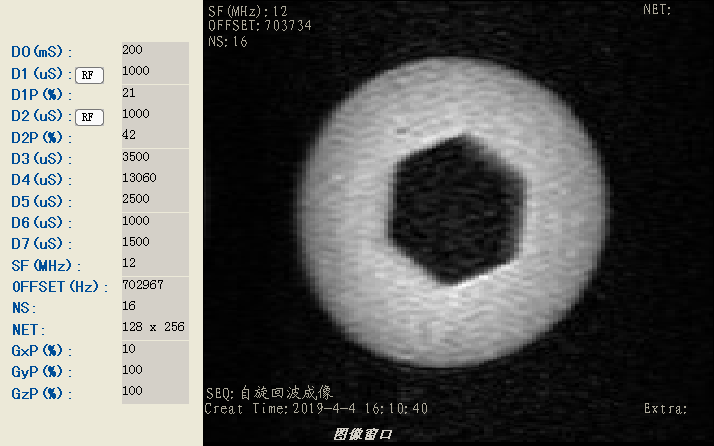
\includegraphics[width=.78\linewidth]{img/plots/sample_hex.png}\\[1ex]
	\caption{\perc{.5} \cuSample 加入正多边形样品后的核磁共振图像以及相应参数}
	\vspace{-2ex}
	\end{figure}
	
	由图可见,正三角形、正六边形各边、角均相当明确,这便验证了该成像方法具有充分高的分辨能力。
	
	为观察到$T_2$加权效应,须改变样品的$T_2$值,这可以通过引入不同浓度的 \cuSample 实现。增大 \cuSample 的浓度,水中质子的浓度$\rho(x,y)$基本不变,而顺磁剂$\mrm{Cu}^{2+}$浓度增大,这使得驰豫时间$T_2$显著减小,对应信号减弱。
\clearpage
	
	实验中,在装有原 \perc{.5} \cuSample 的大试管中嵌入另一装有更高浓度 \cuSample 的小试管以比较$T_2$加权情况,结果如下。
	\begin{figure}[!ht]
	\vspace{1ex}
	\centering\small
	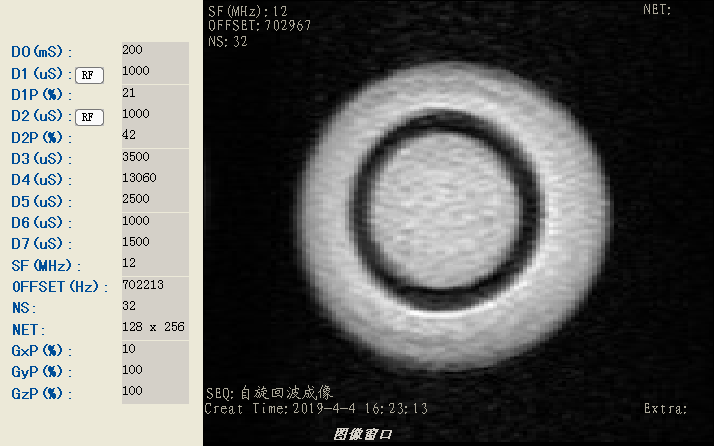
\includegraphics[width=.78\linewidth]{img/plots/sample1.png}\\[1ex]
	(a) \textit{中心小试管:\perc{1} \cuSample}\\[3ex]
	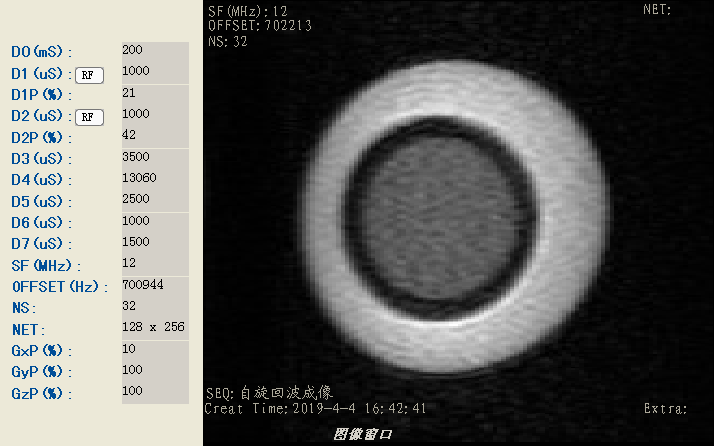
\includegraphics[width=.78\linewidth]{img/plots/sample2.png}\\[1ex]
	(b) \textit{中心小试管:\perc{2} \cuSample}\\[1ex]
	\caption{\perc{.5} \cuSample 加入正多边形样品后的核磁共振图像以及相应参数}
	\vspace{0ex}
	\end{figure}
\FloatBarrier
\clearpage
	
	明显可见中心小试管区域(高浓度)较暗,此即$T_2$加权现象;溶液浓度越大,图像变暗的程度越大。
%	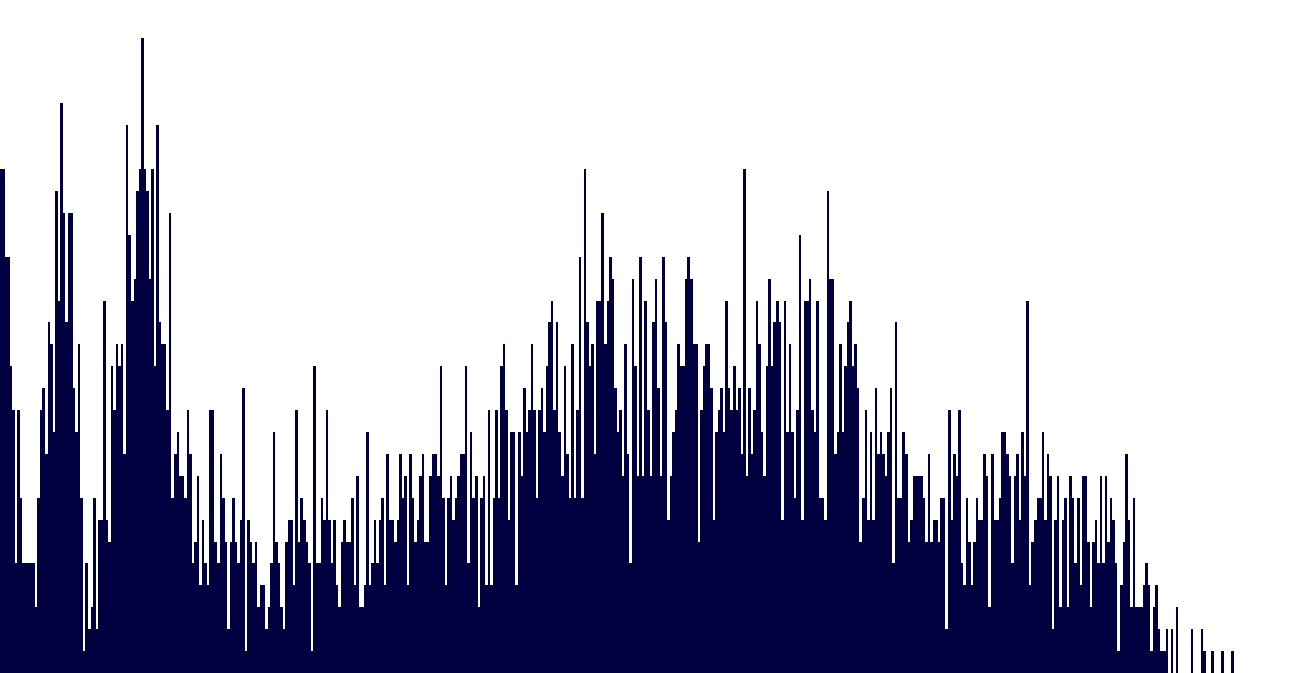
\includegraphics[
%		height=8\baselineskip,
%		width=.8\linewidth,
%		frame
%	]{data/bg_white.png}
%	\begin{table}[!h]
%	\vspace{0\baselineskip}
%	\caption[峰值道址]{参考穆斯堡尔谱的峰值道址}
%	\footnotesize
%	\textit{\tup{(1)} \FeAlpha}\\[1ex]
%	\begin{tabularx}{.85\linewidth}{%
%		C{1} | *6{C{.5}}
%	}
%	\toprule\midrule
%		序号 &
%			1 & 2 & 3 & 4 & 5 & 6 \\
%	\midrule
%		右侧峰道址$v_R$ &
%			289 & 327 & 367 & 396 & 436 & 475 \\
%		左侧峰道址$v_L$ &
%			226 & 186 & 147 & 117 & 77 & 38 \\
%	\midrule\bottomrule
%	\end{tabularx}
%	\label{tab:}
%	\vspace{-.3\baselineskip}
%	\end{table}%
\section{结论}
%%%	首先要给出实验结果,然后再给出由实验结果分析得到的结果和结论。此部分给出的内容要比摘要中的全面,用词要更准确。\par
%%%%%%%%%%%%%%%%%%%%%%%%%%%%%%%
	本实验使用小型核磁共振成像仪获得了 \cuSample 的核磁共振像,利用多边形样品检验了成像的分辨率,并通过比较不同浓度的 \cuSample 验证了$T_2$加权效应;由此加深了对脉冲核磁共振及其成像原理的理解,掌握了小型核磁共振成像仪的基本使用方法。
\section{致谢}
%	此部分感谢同组人...和对实验和报告有帮助的人。
%%%%%%%%%%%%%%%%%%%%%%%%%%%%%%
	感谢黄斐增老师的细致指导和耐心帮助;感谢 \TeX\, - \LaTeX\, Stack Exchange\footnote{%
		\url{https://tex.stackexchange.com/}
	}, 助我解决了众多排版问题。
	
\vspace{1\baselineskip}

\setlength{\bibsep}{2pt}
\linespread{1.2}\selectfont
\bibliographystyle{../BibStyle/gbt-7714-2015-numerical}
\bibliography{../BibStyle/Textbook,bib/Ref}

\clearpage
\end{document}